\section{Исследование и построение решения задачи}
\label{sec:Chapter3} \index{Chapter3}




\subsection{Архитектурное решение}
На основании сравнительного подходов Scala и Kotlin к работе с примитивными типами было принято решение реализовать для рассматриваемого языка стратегию, аналогичную Kotlin:
\begin{itemize}[label={--}]
    \item Все примитивоподобные типы становятся экземплярами Object
    \item Замена на низкоуровневые примитивы выполняется только на этапе оптимизации компиляции
\end{itemize}

Для наглядности далее в тексте в качестве базового примера будут использоваться типы:
int (примитивный) → Int (объектный аналог)

\textbf{Унифицированная система типов предусматривает:}
\begin{enumerate}
    \item Каждый примитивный тип полностью эквивалентен своей объектной обёртке, являющейся подклассом Object
    (включая специальные типы: void/ Void, undefined/ Undefined, null/ Null)
    \begin{itemize}[label={--}]
        \item Арифметические операции выполняются непосредственно с объектами Int без распаковки
        \item Тип Int становится полноценным участником union-типов
        \item Операторы \code{==} и \code{===} реализуют сравнение по значению (аналогично поведению для String)
    \end{itemize}

\end{enumerate}

\newpage
\subsection{Изменения в семантике языка}

\subsubsection{Эквивалентные сценарии}
\begin{figure}[H] % Попробуйте эту комбинацию спецификаторов
    \centering
    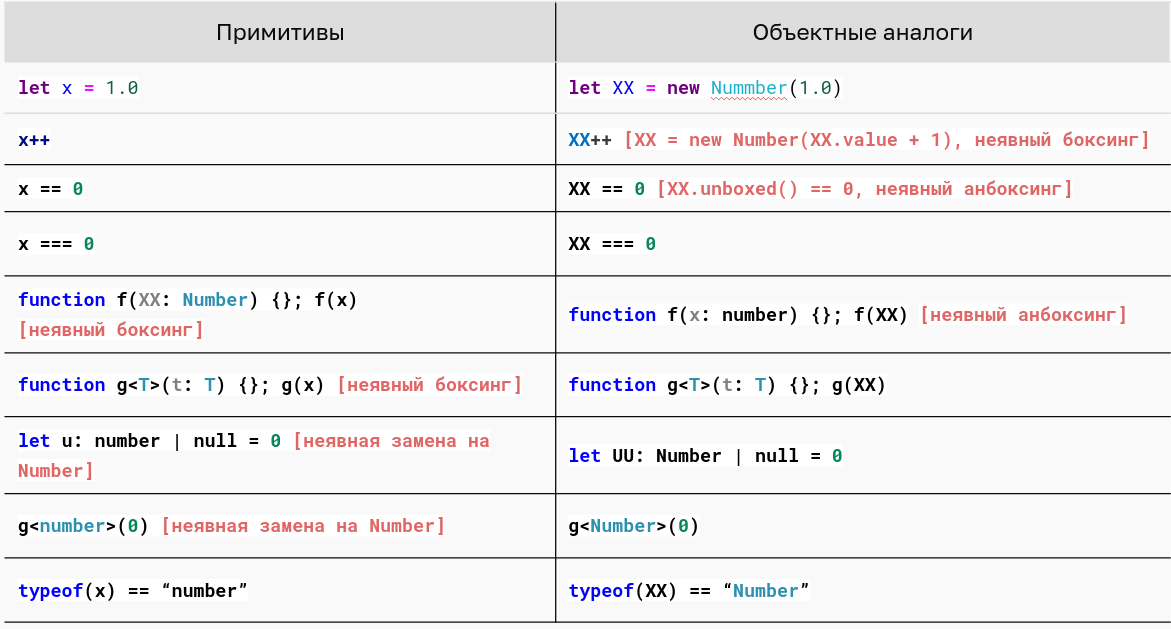
\includegraphics[scale=0.4]{same.png}
    \caption{Красными комментариями помечены места, в которых происходили неявные упаковки и распаковки в ТЕКУЩЕМ языке}
    \label{fig:example}
\end{figure}

\subsubsection{Новые допустимые конструкции}
\begin{figure}[H] % Попробуйте эту комбинацию спецификаторов
    \centering
    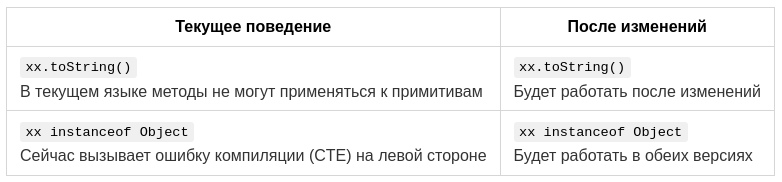
\includegraphics[scale=0.6]{legal.png}
    \caption{Подпись}
    \label{fig:example}
\end{figure}


\subsection{План реализации}
\begin{enumerate}
    \item \textbf{Модификация системы типов}: АУбрать примитивные типы на этапе проверки корректности типов в арифметических операциях и преобразованиях типов
    \item \textbf{Обработка констант}: Изменить представление литералов на этапе свёртки констант на объектные типы
    \item \textbf{Оптимизация перед кодогенерацией}: Имплементировать модуль-оптимизацию, где объектные типы будут по возможности заменяться примитивными
\end{enumerate}

\newpage
